\setcounter{equation}{0}
\chapter{Introduction}

Galaxies are one of the most important structures in the universe. They are key to understand it and its evolution. So far, human kind has been able to study really well our close galaxies. However, the young ones are very far away and only a point of light reaches our telescopes. This point, although tiny, contains information of millions of stars and space material that could unravel many mysteries. For example, it could explain how our own Milky Way  was created. So, it is our challenge as scientists to obtain as much information as possible from it. This task can be fulfilled in many different ways. The purpose of this monograph is to become one of these solutions. \\


\section{Lyman Alpha Emitters}
It has been discovered that young galaxies in the universe are common to have a lot of Hydrogen (H) atoms. Also, that the material inside of them is easily ionized. These two facts leave the H atoms prone to excite.\\

When a Hydrogen atom is excited, the only electron it has moves to a higher energy level. However, a short time passes until it is no longer able to maintain itself in this state. For this, the electron goes back to the ground level it was before. Finally, as the energy obtained from this excitement has to be conserved, it is emitted as a particle of light, called a photon, with a wavelength of 1215.67 $\AA$. This light emission process is called the Lyman Alpha ( \lya) radiation, discovered by Theodore Lyman in 1906.  \\

This \lya radiation happens in all the H atoms in the galaxy. Due to the amount of atoms inside it, the whole body becomes a strong \lya radiator, and the galaxy is now called a Lyman Alpha Emitter (LAE).\\

When astronomers observe a LAE they decompose its incoming light in different wavelengths and make a histogram of them. This distribution is called the spectrum of the galaxy. If now I look at the range of the spectrum around the \lya wavelength there is a clear and strong emission called the \lya line. However, the line is not a single peak at 1215.67 $\AA$ as one would first expect, but it bestrews around this wavelength in a particular shape. This morphology depends mostly on the galaxy's dynamics.\\

\begin{figure}[h!]
	\begin{center}
		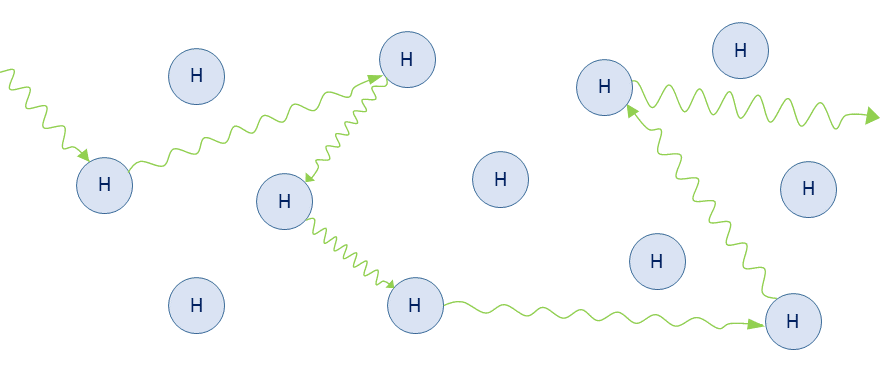
\includegraphics[width=1\textwidth]{./figures/chapter1/radiative_transfer}
	\end{center}
	\caption{\textbf{Radiative Transfer Sketch:} A photon being absorbed and re-emitted by Hydrogen atoms. 
		\label{fig:radiative_transfer}}
\end{figure}

When a photon is emitted, it travels through the interstellar medium (ISM) of the galaxy. During its path it can encounter another H atom and be absorbed by it. The energy carried by the photon is used to excite the atom and start a re-emission process, the same way as described before. This photon's scattering can happen several times until it is able to escape the galaxy, as seen in Fig. \ref{fig:radiative_transfer}. Additionally, as the phenomenon consists of transferring light through scatterings, it is called a radiative transfer process.\\

If the galaxy is completely static, this process would create a single peak around the natural \lya wavelength. Notwithstanding, if now the atoms have a velocity that obeys the dynamics of the galaxy, the re-emitted photon will not have the same wavelength it came with. This is what affects the \lya line shape. \\

These unknown dynamics are what I explore in this work by proposing a new model for a LAE. The model is explained in detail in Chapter \ref{chap:model}. \\


\section{The Radiative Transfer Code}
In order to test this new model I have to know the effect of its parameters in the outgoing \lya line. Nonetheless and on the contrary of other areas of science, in astronomy is not possible to do experiments with the objects we observe. It becomes necessary to draw upon programming to explore and test the new models that appear. Then, with the arrivals of new and better observations these models can be reinforced or refuted in time. \\

In this monograph's case it is then necessary to create a program that simulates a LAE in order to test the model. This means, the code has to take into account the radiative transfer explained in the previous section. This classifies the program as a radiative transfer code. Now, because of the resonant nature of the \lya line, the equation that describes a radiative transfer can not be solved analytically. Numerical methods achieved through computation are required. This remarks how important is for these programs to exist. \\

One radiative transfer code that exists in the literature is CLARA (Code for Lyman Alpha Radiation Analysis). CLARA was created by Forero-Romero et al. \cite{Forero12}. It emulates the \lya line of a spherical rotating LAE depending on its mass and velocity. In this work I modify CLARA so the galaxy behaves as in my model. \\


\section{Monograph Overview}
This monograph is structured as follows. In Chapter \ref{chap:model} I explain the model of rotation and outflows used. In Chapter 3 I present the results of the simulations. In Chapter 4 I compare the results with a LAE observation. In Chapter 5 I present the conclusions and possible future work. Finally, in the Appendix, I present the results of a \lya line modeled also with rotation and outflows but with a different implementation. \\



